
\chapter{La s\'ecurit\'e dans le monde de l'automobile} \label{CHAP2}
\smallskip
\hfill
\begin{minipage}[b]{8cm}
{\it Ce travail f\^ut pr\'esent\'e en partie \`a la conf\'erence des sourds-muets unijambistes \`a Quib\'eron en avril 1994.}
\end{minipage}
\begin{flushright} Maxime Ayrault \end{flushright}
\vskip 2cm

\section {La r\'evolution logicielle}
\medskip
{\Huge L}e logiciel embarqu\'e est une des innovations cl\'e dans le monde automobile.
D'apr\`es l'article de Robert Charette (\cite{Cha2009}) paru dans IEEE Spectrum, la premi\`ere voiture embarquant un logiciel \'etait la Oldsmobile Toronado de General Motors en 1977. La Toronado avait une unit\'e de contr\^ole \'electronique (ECU) qui g\'erait la synchronisation de l'allumage des bougies (spark timing). En 1978, General Motors proposait, en option sur ses Cadillacs, un ordinateur de bord qui pouvait afficher la vitesse, le niveau du r\'eservoir d'essence, les informations sur l'\'etat du v\'ehicule. Ce logiciel s'ex\'ecutait sur une version modifi\'ee du processeur Motorola 6802 et faisait 50.000 lignes de code. Depuis, de plus en plus de fonctions ont \'et\'e r\'ealis\'ees par du logiciel. Afin de limiter le nombre de c\^ables dans une voiture, les capteurs ont \'et\'e d\'ecentralis\'es et connect\'es \`a un r\'eseau interne (r\'eseau CAN). Le logiciel a \'egalement permis de cr\'eer de nouvelles fonctions pour les voitures. \\
Une voiture actuelle est maintenant devenue une plate-forme logiciel sur roues. Une voiture grand public contient entre 30 et 50 unit\'es de contr\^ole \'electronique effectuant la gestion de multiples syst\`emes (voir \ref{tab:soft}).

\FloatBarrier
\begin{table}
\centering
\begin{tabular}{| l | l | l |}
\hline
Air bag & ABS & Syst\`eme d'alarme \\
\hline
La climatisation & Le r\'egulateur de vitesse & Le r\'egime moteur \\
\hline
Les clignotants & Les feux & Le klaxon \\
\hline
La gestion des si\`eges & Le syst\`eme de navigation & Le syst\`eme audio \\
\hline
La pression des pneus & La gestion des portes et vitres & ... \\
\hline
\end{tabular}
\caption{Syst\`eme logiciel dans une voiture}
\label{tab:soft}
\end{table}
\FloatBarrier


En 2009, Alfred Katzenbach, le directeur des Technologies Informatique Chez Daimler, a annon\c c\'e que le syst\`eme navigation et audio sur une Mercedes-Benz  S-class contient plus 20 millions de lignes de code et que la voiture contienait pratiquement autant d'unit\'e \'electronique qu'un Airbus A380 (si on exclut le syst\`eme de divertissement en vol) (\cite{Cha09}).  Les logiciels dans une voiture grossissent \`a une vitesse exponentielle en taille et en complexit\'e. En 2010, certaines voitures avaient 10 millions de lignes de code. En dix ans, le volume du logiciel a augment\'e par un facteur 15, pour environ 150 millions de lignes. Aujourd'hui, le Model S de Tesla est \'equip\'ee d'un \'ecran tactile de 17 pouces bas\'e sur un syst\`eme d'exploitation Linux qui contr\^ole quasiment toute les fonctions utilisateurs de la voiture. En fait, il n'y a plus que 2 boutons manuel non g\'er\'es par du logiciel sur un Model S; le bouton pour les feux de d\'etresse et le bouton de la bo\^ite \`a gants. \\

Un effet secondaire est sur la complexit\'e des fonctions propos\'ees aux conducteurs. Il n'est pas rare que les manuels utilisateurs des voitures fassent maintenant plus de 500 pages pour expliquer l'ensemble des fonctions logiciel. D'un autre c\^ot\'e, on estime qu'un conducteur moyen n'utilise pas plus de 20\% des fonctions impl\'ement\'ees par du logiciel. Les constructeurs automobiles commencent \`a se poser la question sur une limitation des fonctions r\'ealis\'ees par du logiciel. Par exemple, est-il vraiment n\'ecessaire que la lumi\`ere du plafonnier d'une voiture s'\'eteigne de fa\c con progressive?\\

L'augmentation du logiciel a \'egalement d'importantes cons\'equences sur la fa\c con d'entretenir et de r\'eparer une voiture. On estime que plus de 50\% des unit\'es \'electroniques remplac\'ees n'ont pas d'erreur (logiciel ou mat\'eriel). Le garagiste remplace fr\'equemment une pi\`ece car il ne sait pas quelle est la cause principales de la panne. La principale activit\'e des garagiste consiste \`a t\'e\'echarger les nouvelles versions du logiciel. Sur les voitures Tesla, les mises \`a jour logiciel, qui incluent les corrections du logiciel et les nouvelles fonctionnalit\'es sont t\'el\'echarg\'ees dans la voiture via le r\'eseau cellulaire sans intervention d'un garagiste.\\  

Aujourd'hui, le co\^ut du logiciel et de l'\'electronique repr\'esente entre 35 \`a 40\% du co\^ut d'une voiture. \\


\begin{tbd}
Introduire Automotive Open System Architecture (AUTOSAR). Une solution pour r\'eduire le co\^ut du logiciel en augmentant l'interop\'erabilit\'e entre les constructeurs.
\end{tbd}


L'introduction du logiciel a permis d'avoir des voitures plus s\^urs et moins polluantes mais a \'egalement introduit une nouvelle menace; la \emph{s\'ecurit\'e informatique des voitures}. 

\section {Architecture voiture}

\begin{tbd}
Commencer a pr\'esenter les diff\'erentes couches logiciel.\\

the following four stacks could become the basis for upcoming generations of cars in five to ten years:
\begin{itemize}

\item \emph{Time-driven stack}. In this domain, the controller is directly connected to a sensor or actuator while the systems have to support hard real-time requirements and low latency times; resource scheduling is time based. This stack includes systems that reach the highest Automotive Safety Integrity Level classes, such as the classical Automotive Open System Architecture (AUTOSAR) domain.
\item \emph{Event- and time-driven stack}. This hybrid stack combines high-performance safety applications, for example, by supporting ADAS and HAD capability. Applications and peripherals are separated by the operating system, while applications are scheduled on a time base. Inside an application, scheduling of resources can be based on time or priority. The operating environment ensures that safety-critical applications run on isolated containers with clear separation from other applications within the car. A current example is adaptive AUTOSAR.
\item \emph{Event-driven stack}.This stack centers on the infotainment system, which is not safety critical. The applications are clearly separated from the peripherals, and resources are scheduled using best-effort or event-based scheduling. The stack contains visible and highly used functions that allow the user to interact with the vehicle, such as Android, Automotive Grade Linux, GENIVI, and QNX.
\item \emph{Cloud-based (off-board) stack}. The final stack covers and coordinates access to car data and functions from outside the car. The stack is responsible for communication, as well as safety and security checks of applications (authentication), and it establishes a defined car interface, including remote diagnostics.
\end{itemize}

\url{https://www.mckinsey.com/industries/automotive-and-assembly/our-insights/rethinking-car-software-and-electronics-architecture}
\end{tbd}


\FloatBarrier
\begin{figure}
    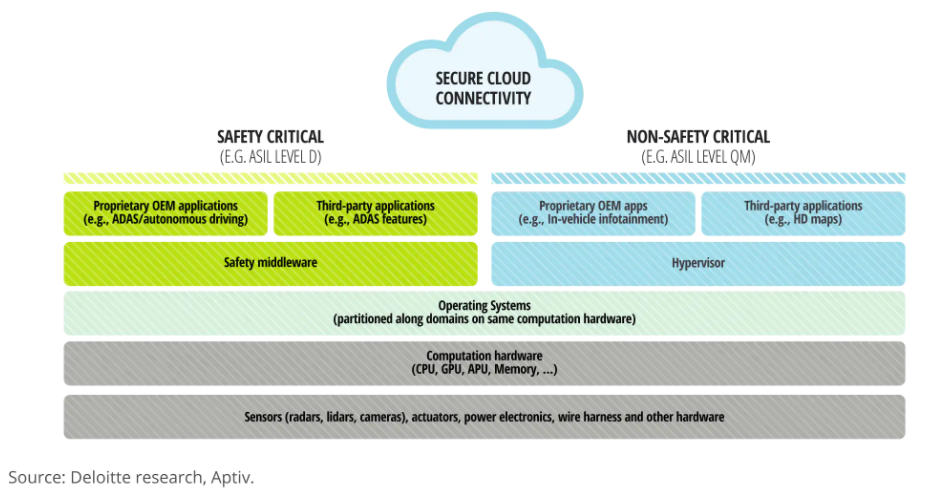
\includegraphics[width=\textwidth]{architecture}
    \caption{Architecture g\'en\'erique}
    \label{fig:archi}
\end{figure}
\url{https://www2.deloitte.com/us/en/insights/focus/future-of-mobility/pure-play-software-in-automotive-industry.html}
\FloatBarrier

Bla bla bla


\section {Principes de la s\'ecurit\'e informatique}
\medskip
{\Huge L}a s\'ecurit\'e informatique est construite sur 3 piliers (CIA triad).
  
\begin{itemize}
\setlength\itemsep{1em}
\item La \emph{confidentialit\'e}. L'objectif consiste \'a \'eviter la divulgation d'informations sensibles et/ou de prot\'eger les acc\`es non authoris\'es ressources sensibles. Autrement dit, la confidentialit\'e implique la protection des donn\'ees (resp. ressources), en donnant acc\`es \`a ceux qui sont autoris\'es \`a les lire (resp. \`a les utiliser) tout en interdisant aux autres d'apprendre quoi que ce soit sur son contenu (ou son existence).  
\item L'\emph{int\'egrit\'e}. L'objectif est de prot\'eger ou de minimiser les modifications non authoris\'ees de donn\'ees et/ou ressources sensibles. Autrement dit, l'int\'egrit\'e implique de pr\'eserver le contenu des donn\'ees et de d\'etecter si une donn\'ee ou une ressource a \'et\'e alt\'er\'ee depuis sa derni\'ere \'ecriture par une personne authoris\'ee.  
\item La \emph{disponibilit\'e}. L'objectif est de maintenir le syst\`eme op\'erationel pour rendre le service aux l'utilisateurs.  
\end{itemize}

\FloatBarrier
\begin{figure}[h]
	\centering
    \includegraphics[scale=1.0]{CIA-triad}
    \caption{Les pilers de la s\'ecurit\'e informatique}
    \label{fig:CIA}
\end{figure}
\FloatBarrier


Les principales techniques utilis\'ees pour garantir ces 3 propri\'et\'es sont:
\begin{itemize}
\setlength\itemsep{1em}
\item \emph{Chiffrement (Encryption)}: La transformation de l'informations originale (appel\'e clair) \`a l'aide d'une cl\'e de chiffrement, de telle sorte que les informations transform\'ees (appel\'e chiffr\'e) ne puissent \^etre interpr\'et\'ees que par un autre utilisateur ayant connaissance de la cl\'e de d\'echiffrement (qui peut, dans certains cas, \^etre identique \`a la cl\'e de chiffrement). Pour \^etre en s\'ecurit\'e, un algorithme de chiffrement doit rendre extr\^emement difficile pour quelqu'un de d\'eterminer tout ou partie des informations clairs sans connaissance de la cl\'e de d\'echiffrement ou faiblesse de l'algorithme de chiffrement. 

\item \emph{Authentification (Authentication)}: La d\'etermination de l'identit\'e qu'un sujet (personne, logiciel ou \'equipement). Cette d\'etermination peut \^etre effectu\'ee par plusieurs moyens. Il est g\'en\'eralement bas\'e sur une combinaison de quelque chose que la personne conna\^it (Something you know) comme un mot de passe ou un code PIN, quelque chose le sujet poss\`ede (Something you have) comme une carte \`a puce contenant des cl\'es secr\`etes un t\'el\'ephone pour recevoir un code, un passeport, ou quelque chose la personne est (Something you are) comme une empreinte digitale.

\item \emph{Contr\^oles d'acc\`es (Access Control)}: Ensemble de r\`egles et politiques de s\'ecurit\'e qui limitent l'acc\`es aux informations aux sujets (personnes et/ou syst\`emes) ayant un \emph{besoin d'en connaitre}. Ce besoin d'en connaitre est d\'etermin\'e suite \`a l'authentification correcte du sujet, de par son identit\'e ou r\^ole. Un ensemble de r\`egles est pr\'e-d\'efinie par le gestionnaire de la s\'ecurit\'e informatique en se basant sur la politique de s\'ecurit\'e.

\item \emph{Signature (Signature)}: La signature d'une information a deux objectifs; assurer que l'information sign\'ee n'a pas \'et\'e alt\'er\'ee depuis la signature et authentifier la source de l'information (non-repudiation). La signature consiste en un chiffre d\'ependant d'une cl\'e secr\`ete connue uniquement par le sujet signant l'information et du contenu du message \`a signer. Une signature est v\'erifiable, sans connaitre la cl\'e secr\`ete, par une partie tierce en cas de litige entre parties. Si le contenu du message ou la signature est modifi\'e, la correspondance entre le contenu initial et message et sa signature sera invalide permettant de d\'etecter l'alt\'eration et de rejecter l'information. De fa\c con, sym\'etrique, si le contenu du message et sa signature correspondent alors la source de l'information ne pourra pas nier avoir sign\'e l'information car elle est la seule \`a connaitre la cl\'e secr\`ete.

\item \emph{Responsabilit\'e (Accountability)}: La capacit\'e de rendre le sujet responsable de ces actions. Ceci est r\'ealis\'e en s'appuyant sur des journaux d'audit (audit log). Une fois le sujet correctement authentifi\'e, toutes ces actions sont enregistr\'ees sous forme d'\'ev\'enements dans un journal d'audit. En cas d'investigation ou de fa\c con p\'eriodique, le gestionnaire de la s\'ecurit\'e informatique peut r\'ealiser un audit des journaux pour identifier la source potentielle d'une attaque.

\item \emph{Sensibilisation \`a la s\'ecurit\'e (Security awareness)}: La principale source de risque pour une organisation ne provient pas de faiblesse dans la technologie des \'equipements mais d'actions (ou d'inaction) de la part des utilisateurs du syst\`eme. Afin de limiter ce risque, il est n\'ecessaire de former les utilisateur aux diif\'erents risques informatiques et aux bonnes pratiques pour assurer le niveau de s\'ecurit\'e requis. 

\item \emph{S\'ecurit\'e physique (physical security)}: Mise en place de barri\`eres physiques pour limiter l'acc\`es aux ressources sensibles. Ces barrières comprennent sont mutiples comme le gardiennage, la vid\'eo-surveillance, les serrures sur les armoires et les portes, les chambres fortes, l'utilisation de matériaux insonorisants, ou m\^eme la construction d'\'equipement renforc\'e (tempest) afin que les signaux \'electromagn\'etiques ne puissent pas entrer ou sortir.

\item \emph{Tol\'erance aux fautes (fault tolerance)}: Ensemble de techniques peuvent \^etre utilis\'ees pour garantir le syst\'eme en op\'eration.
\end{itemize}


\FloatBarrier
\begin{table}[h]
\centering
\begin{tabular}{| l | c | c | c |}
\hline
& Confidentialit\'e & Integrit\'e & Disponibilit\'e \\
\hline
Chiffrement & \checkmark & &  \\
\hline
Authentification & \checkmark & \checkmark &  \\
\hline
Contr\^oles d'acc\`es & \checkmark & \checkmark &  \\
\hline
Signature &  & \checkmark &  \\
\hline
Responsabilit\'e & \checkmark & \checkmark &  \\
\hline
Sensibilisation \`a la s\'ecurit\'e physique & \checkmark & \checkmark & \checkmark \\
\hline
S\'ecurit\'e physique & \checkmark & \checkmark & \checkmark \\
\hline
Tol\'erance aux fautes & & & \checkmark \\
\hline
\end{tabular}
\caption{Principales m\'ethodes de la s\'ecurit\'e informatique}
\label{tab:cia}
\end{table}
\FloatBarrier


Dans le reste de la th\`ese, nous concentrerons sur la disponibilit\'e des syst\`emes embarqu\'es. 


\section {Le risque cybers\'ecurit\'e pour l'automobile}
 \medskip
 {\Huge L}'ajout de logiciels et de connectivit\'e....


3 niveaux d'attaques:
\begin{itemize}
\setlength\itemsep{1em}
\item \emph{Attaques physiques}. 
\begin{itemize}
\item Attaque via la prise diagnostique de la voiture. L'objectif est de pouvoir modifier les caract\'eristiques de la voiture et/ou de rajouter des options sur la voiture. Les logiciels d'une voiture sont hautement configurables. Un m\^eme logiciel est install\'e sur plusieurs gammes de v\'ehicules d'un constructeur. La diff\'erenciation entre les deux mod\`eles s'effectue par le param\'trage du logiciel. Si un attaquant \`a la possibilit\'e de modifier ces param\`etres, il peut activer des fonctions optionnelles de la voiture ou modifier les caract\'eristiques moteur pour booster le v\'ehicule.
\item Attaque via la prise USB de la voiture. L'objectif est de pouvoir cr\'eer un point d'entr\'ee pour une attaque courte ou longue port'ee sur le v\'ehicule. La prise USB peut \^etre connect\'ee sur un \'equipement radio qui permet d'\'etendre la port\'ee de l'attaque.
\end{itemize}

\item \emph{Attaque courte port\'ee} L'objectif est de pouvoir prendre le contr\^ole du v\'ehicule, d'envoyer de fausses informations ou de bloquer les communicatiosn aux v\'ehilcules aux alentours. De plus en plus de voitures ont un syst\`eme d'ouverture de portes et de d\'emarrage sans cl\'e.Par exemple, votre voiture est gar\'ee devant votre maison et les cl\'es sont sur le petit d'entr\'ee.  Un attaquqant peut ins\'erer un \'equipement radio entre la cl\'e et la voiture (attaque par relais). Un c\^ot\'e est proche de la voiture, lautre c\^ot\'e est connect\'e \`a une antenne scannant les fr\'equences radio de la cl\'e. Ceci permet d'ouvrir et/ou de d'emarrer la voiture m\^eme quand les cl\'es du v\'ehicule sont hors de port\'ee de la voiture. Une fois que l'antenne a accroch\'e la fr\'equence de la cl\'e, elle relaye son signal sur l'\'equipement proche du v\'ehicule. La voiture a ainsi l'impression que le propri\'etaire est proche et ouvre les portes et autorise la d\'emarrage. Le v\'ehicule peut \^etre vol\'e sans effraction (voir \url{https://www.youtube.com/watch?v=_cua7BFX-Qk} pour un video d'attaque relais). Un autre exemple, consiste \`a brouiller le signal pour la fermeture centralis\'ee d'un v\'ehicule. Le conducteur appuie sur le bouton de fermeture centralis\'ee de sa cl\'e, il a le sentiment que sa voiture est correctement ferm\'ee. Mais si le signal est brouill\'e, la voiture est ouverte et un attaquant peut facilement ouvrir un porte pour voler des affaires dans la voiture.
 
\item \emph{Attaque longue port\'ee}. L'objectif est de prendre le contr\^ole \`a distance d'un v\'ehicule. Un des fameux exemple de ce type d'attaque est la prise de contr\^ole d'une Jeep Cherokee par 2 attaquants; Andy Greenberg conduisait sa voiture sur l'autoroute vers Saint-Louis, roulant \` 70 mph. 2 hackers Charlie Miller et Chris Valasek sont install\'es dans leur canap\'e avec leur laptop ouvert. Dans un premier temps, la climatisation de la voiture s'est affol'ee, puis, une image des 2 hackers est apparue sur l'\'ecran de la voiture, la radio a chang\'e de station et le volume a fortement augment\'e, Mr Greenberg ne pouvait pas contr\^oler le volume de la radio ni la station. Ensuite la voiture s'est arr\^et\'ee toute seule. (voir \cite{Mil2015} pour le d\'etail de l'attaque)
\end{itemize}

